\section{Liczniki synchroniczne}

\subsection{Zadanie}

Zaprojektować licznik synchroniczny realizujący liczenie w postaci $0 \rightarrow
2 \rightarrow 1 \rightarrow 3 \rightarrow 7 \rightarrow 6 \rightarrow 9$. Układ zostanie zrealizowany na przerzutnikach JK - Jebać Kleksa ))))
\\
W tym zadaniu najlepiej sprawdza się instrukcja doktora Antoniego Sterny, polecam przeczytać bo jest gitówa. 

\subsection{Tabela przejść}

\begin{figure}[h!]
    \centering
    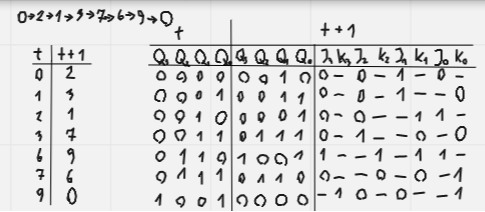
\includegraphics[width = 12cm]{images/sync/sync_t.png}
    \caption{Tabela przejść}
    \label{fig:my_label}
\end{figure}

\subsection{Siatki Karnaugh}

\begin{figure}[h!]
    \centering
    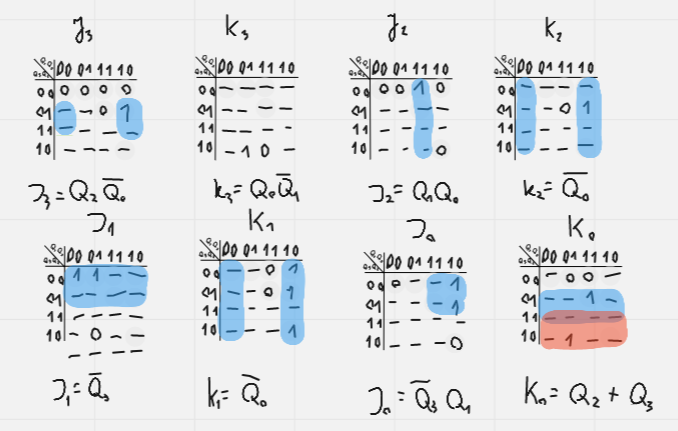
\includegraphics[width = 12cm]{images/sync/sync_k.png}
    \caption{Siatki Karnaugh}
    \label{fig:my_label}
\end{figure}

\newpage

\subsection{Schemat układu}

\begin{figure}[h!]
    \centering
    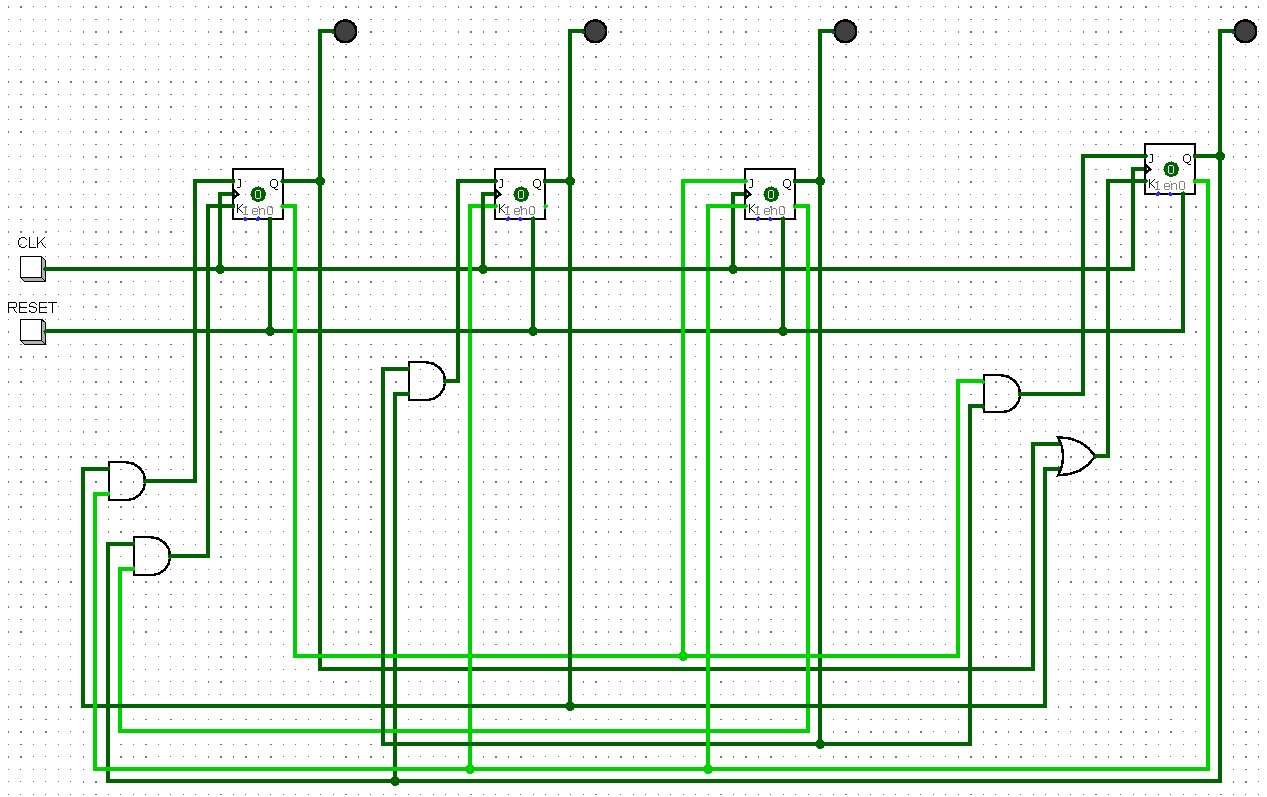
\includegraphics[width = 12cm]{images/sync/sync_l.png}
    \caption{Schemat układu}
    \label{fig:my_label}
\end{figure}

\subsection{Klik}

\url{http://staff.iiar.pwr.wroc.pl/antoni.sterna/luc/LUC_synteza_licznikow.pdf}
